\noindent En este capítulo se abordan los trabajos relacionados con el tema de análisis y detección de amenazas de malware y ransomware mediante el uso de algoritmos de aprendizaje automático y otras técnicas mencionadas en el Capítulo \ref{Capitulo3}. Se describirá cómo han creado sus modelos de \gls{ML} y qué resultados han obtenido. Se realiza una distinción entre los estudios cuya finalidad es la detección de malware \ref{sec:trabajosmalware} y aquellos para el análisis de ransomware \ref{sec:trabajosransom}. Al final del capítulo se mostrará una tabla con los trabajos relacionados y los resultados detallados.

\section{Trabajos sobre Análisis de Malware} 
\label{sec:trabajosmalware}

\noindent Konrad Rieck \textit{et al.} (2011) \cite{automatic} proponen un \textit{framework} (entorno o marco de trabajo) para analizar mediante el aprendizaje automático el comportamiento de malware. Este marco permite identificar nuevas clases de malware con un comportamiento parecido (\textit{clustering} o agrupamiento) y asignarlas en una estas clases (clasificación). En la Figura \ref{fig:automatic} se muestra una descripción esquemática de este marco de análisis. Exponen un enfoque para el análisis basado en el comportamiento que puede procesar miles de archivos de malware a diario en un entorno seguro usando CWSandbox. Proponen un mapeo del comportamiento en un espacio vectorial, de modo que los patrones de comportamiento sean accesibles de manera eficiente por las técnicas de aprendizaje automático. El comportamiento que coincide con el de malware conocido se identifica mediante vectores prototipo de clústeres previamente descubiertos, y posteriormente los informes que contienen el comportamiento no identificado se agrupan para descubrir nuevos tipos de malware. Usan dos conjuntos de datos para los experimentos, uno que contiene 3.133 muestras de malware conocido sacado de la página web de CWSandbox, y otro con 33.698 muestras desconocidas obtenidas de Sunbelt Software. Limitan las muestras de cada tipo de malware a 300, las analizan usando CWSandbox, y esto da como resultado 3.133 informes de comportamiento. Su \textit{framework} reduce los requisitos de memoria en un 94\% con un factor de aceleración de 4, lo que permite procesar 33.000 informes de comportamiento de malware en menos de 25 minutos, algo que superaba a los métodos de análisis más avanzados en su día. En los experimentos con uno de los prototipos obtienen una exactitud (\textit{precision}) del 99,6\% y un valor-F (\textit{F-score}) del 95\%.

\begin{figure}[h!]
\begin{center}
{\scalebox{.26}{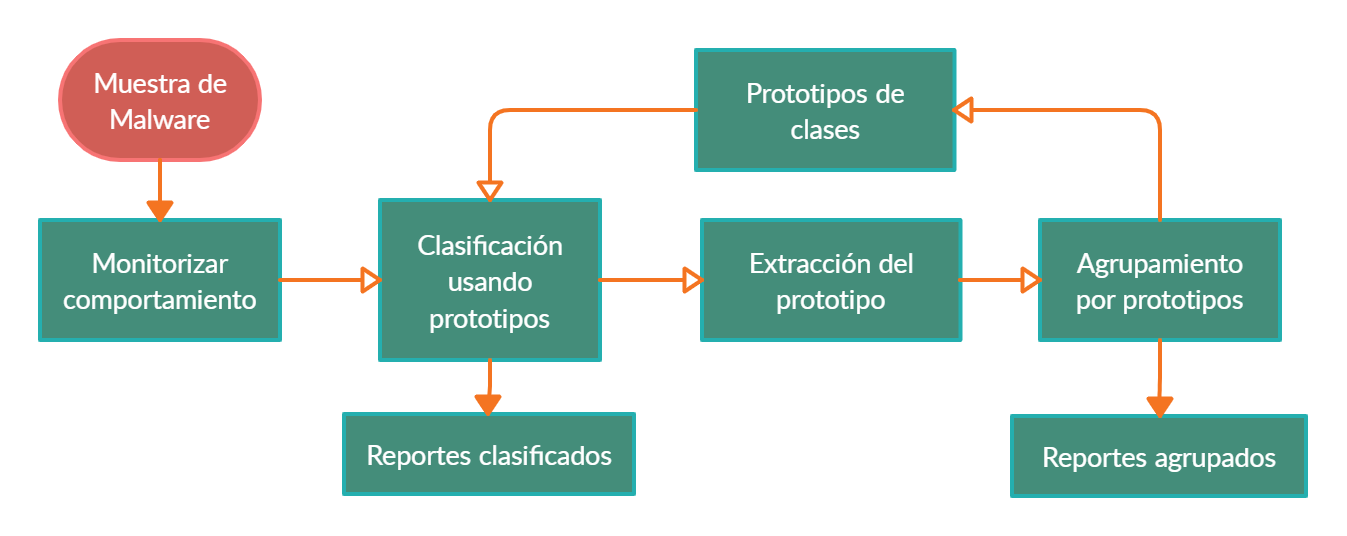
\includegraphics{images/automatic.png}}}
\end{center}
\caption{Descripción esquemática del marco de análisis de Konrad Rieck \textit{et al.}}
\label{fig:automatic}
\end{figure}

\newpage

Mamoun Alazab \textit{et al.} (2011) \cite{zero} proponen un sistema que emplea varias técnicas de minería de datos para detectar y clasificar malware en función de la frecuencia de las llamadas a la \gls{API} de Windows. La metodología general que siguen es la mostrada en la Figura \ref{fig:zero}, donde primero desempaquetan el malware, extraen las \gls{API} y analizan su comportamiento, comparando los resultados con una base de datos de firmas. Después de haber extraído las mejores características, crean el modelo de aprendizaje supervisado para clasificar la muestra (malware o benigno), utilizando algoritmos como \gls{NB}, \gls{KNN}, \gls{DT} y \gls{SVM} con 4 diferentes núcleos. Utilizan la validación cruzada de k iteraciones (\textit{K-fold cross-validation}) para evaluar los resultados del análisis con k = 10. El conjunto de datos consta de 51.223 muestras de malware sacadas de VX Heaven y Honeynet y 15.480 muestras de software benigno. El sistema consigue una tasa de verdaderos positivos (\gls{TPR}) de más del 98,5\% y una tasa de falsos positivos (\gls{FPR}) de menos del 2,5\%, algo que no se había logrado antes.

\begin{figure}[h!]
\begin{center}
{\scalebox{.23}{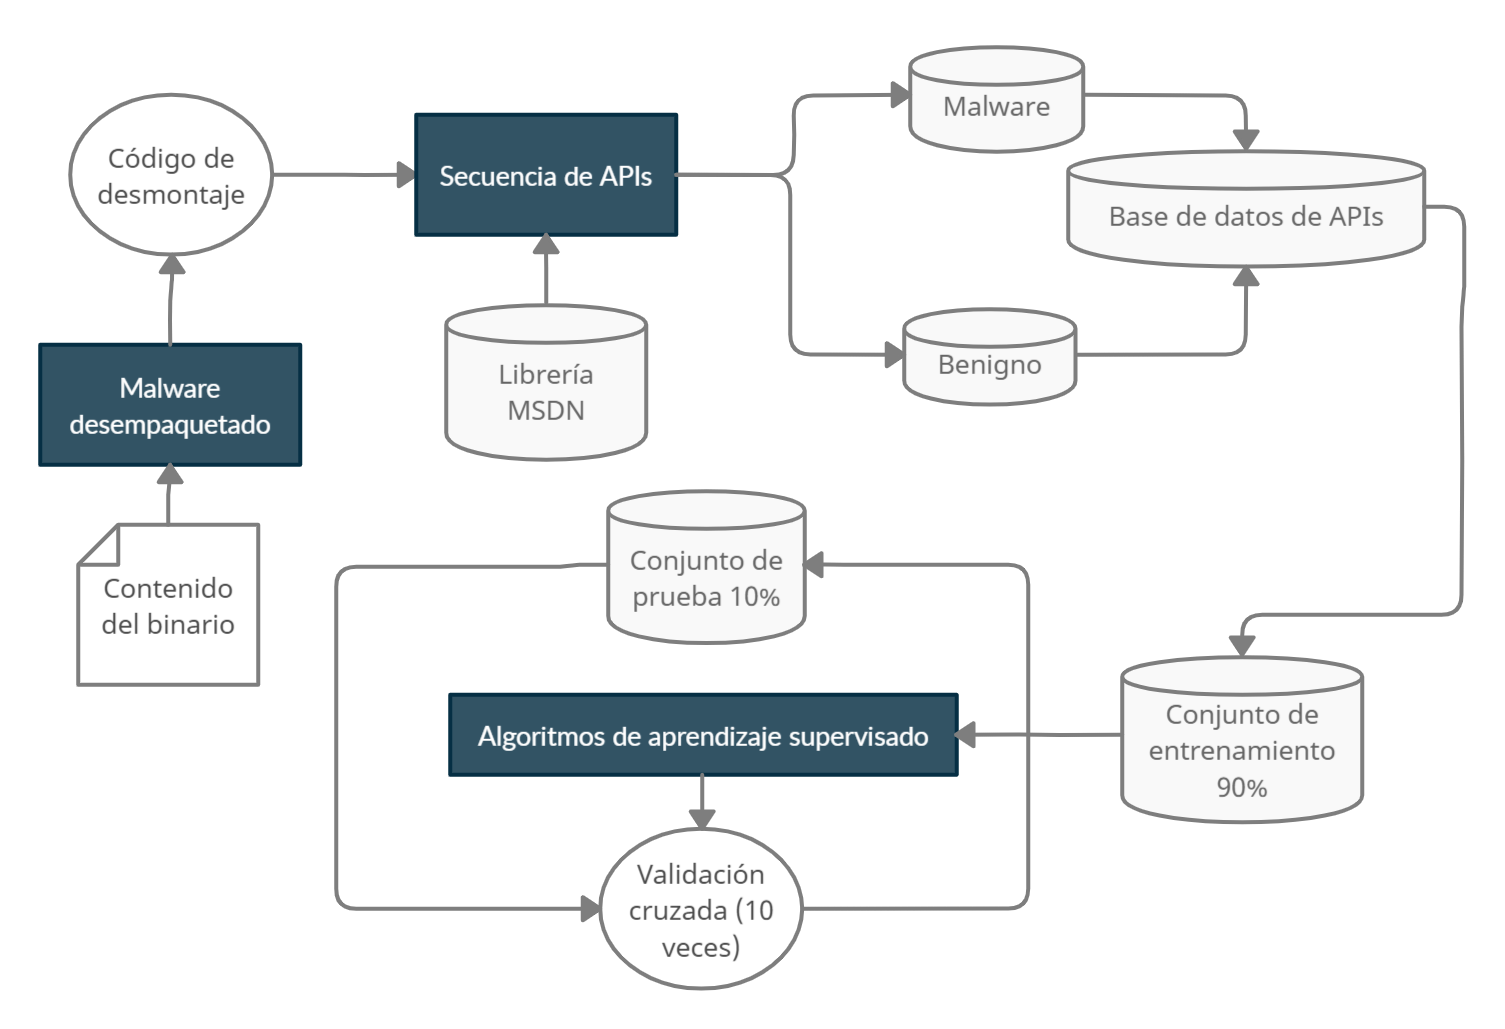
\includegraphics{images/zero.png}}}
\end{center}
\caption{Metodología general del sistema usado en el trabajo de Mamoun Alazab \textit{et al.}}
\label{fig:zero}
\end{figure}


Chandrasekar Ravi \textit{et al.} (2012) \cite{ravimalware} proponen un sistema de detección de malware que modela la secuencia de llamadas de la \gls{API} de Windows con una cadena de Markov de tercer orden. La Figura \ref{fig:ravi} es una representación de la arquitectura de este sistema. Usan algoritmos de clasificación basados en asociación y monitorizan un subconjunto mínimo de categorías de \gls{API} para asegurar la eficiencia del sistema. La novedad que introducen es el proceso de aprendizaje iterativo combinado con la monitorización del comportamiento del programa sospechoso en tiempo de ejecución, creando un sistema dinámico de detección de malware que consta de 3 fases de aprendizaje: offline, online e iterativo. La fase offline están constituida por los siguientes componentes: un conjunto de datos (\textit{dataset}), un rastreador de llamadas de las \gls{API}, una base de datos con los índices de las \gls{API}, una base de datos de firmas, un generador de reglas y una base de datos de reglas. El conjunto de datos contiene 179 muestras de varios tipos de malware y 94 programas benignos. La fase online consta de: el proceso sospechoso que se va a analizar, un rastreador de llamadas de las \gls{API} para ese proceso en específico, una base de datos con los índices de las \gls{API} y el clasificador. El clasificador asigna una etiqueta (benigno o malware) al proceso, utilizando la secuencia rastreada de llamadas a las \gls{API} y las reglas generadas en la fase offline. En la fase iterativa, después de cada clasificación, la etiqueta asignada y la secuencia de las \gls{API} del proceso analizado se agregan iterativamente a la base de datos de firmas. Esto mejorará el modelo de entrenamiento al tener más información para comparar con otros procesos en el futuro. El rendimiento de este sistema supera a los sistemas de detección de malware existentes de la época, con una precisión (\textit{accuracy}) del 90\%.

\begin{figure}[h!]
\begin{center}
{\scalebox{.33}{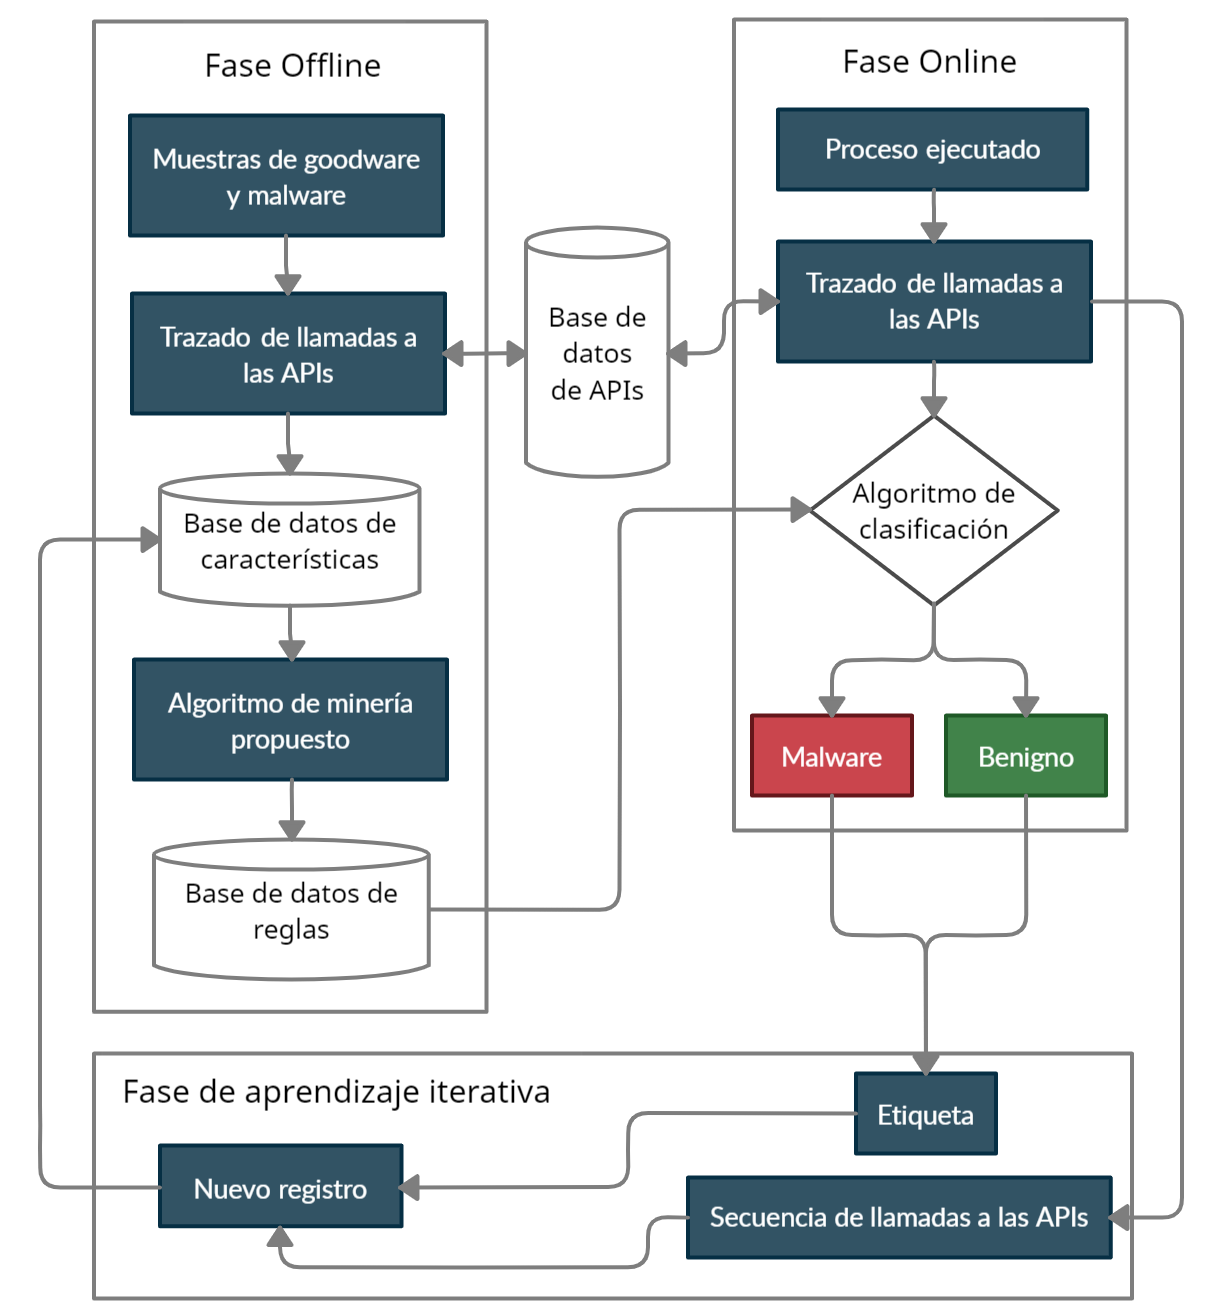
\includegraphics{images/ravimalware.png}}}
\end{center}
\caption{Arquitectura del sistema de detección de malware propuesto por Chandrasekar Ravi \textit{et al.}}
\label{fig:ravi}
\end{figure}


\section{Trabajos sobre Análisis de Ransomware}
\label{sec:trabajosransom}
\subsection{Trabajos que Utilizan Características Heterogéneas}
\noindent En esta sección se agrupan diversos trabajos con métodos heterogéneos para la detección de ransomware distintos a los que se van a utilizar en este estudio, pero de los cuales se puede obtener información relevante.

Amin Kharaz \textit{et al.} en \cite{197235} (2016) realizan un estudio analizando 148.223 muestras de malware reciente, mostrando que el sistema es capaz de detectar correctamente 13.367 muestras de ransomware de diferentes familias, 7.572 de ellas eran desconocidas previamente y no habían sido detectadas por ningún antivirus. 

Se trata de una aplicación que se acopla al sistema al driver del sistema de ficheros, permitiendo su monitorización. 
Además, se combina con la creación de un entorno artificial, que detecta cambios en el escritorio para la detección de ransomware Lockscreen. Este ha de ser lo más realista posible: los datos tienen que ser reales, válidos y no deterministas para no ser reconocidos por los atacantes. Para cada extensión de archivos presente en el sistema de usuario, se crean un número aleatorio de archivos con cabeceras válidas y contenido usando bibliotecas estándar y \textit{queries} de palabras en inglés obteniendo 100.000 frases distintas. Al igual se tiene precaución a la hora de crear los directorios y su estructura de forma realista y no determinista. Se lleva a cabo un algoritmo estadístico para establecer las fechas de creación, modificación y acceso.
En cuanto a la monitorización de sistema de archivos se observa que existen patrones repetidos, usan diferentes estrategias para evitar el acceso a los archivos, hay tres patrones diferenciados que aparecen en la Figura \ref{fig:im12}. Se comprueba la entropía de los archivos en las operaciones de entrada y salida, en lugar de las llamadas a la \gls{API} de Windows, para saber si están siendo cifrados. Se realiza mediante el \textit{framework} Windows Filesystem Minifilter Driver, del kernel de Windows. Esto permite que Unveil este localizado en la capa más cercana posible al \textit{Filesystem}.

\begin{figure}[h!]
\begin{center}
{\scalebox{.825}{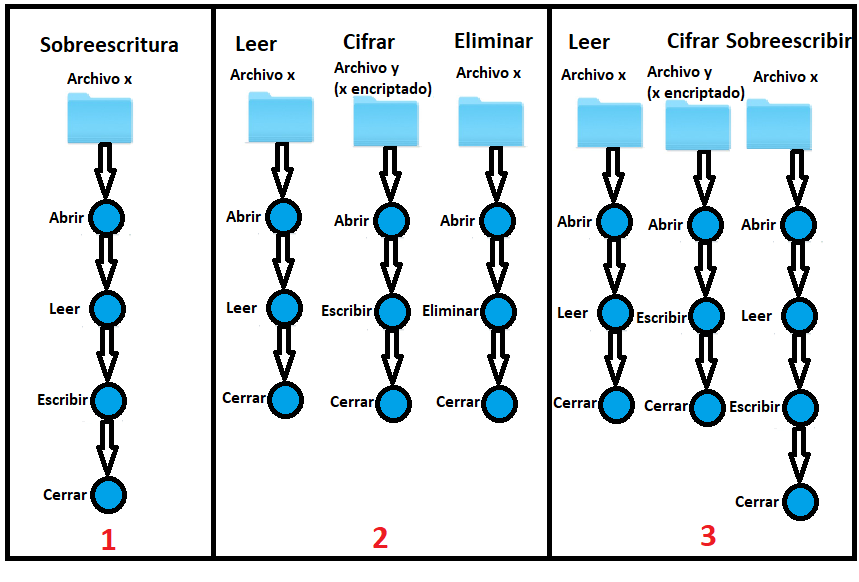
\includegraphics{images/unveil2.png}}}
\end{center}
\caption{Patrones del ransomware para cifrar archivos: 1- El atacante sobrescribe el fichero del usuario con la versión cifrada. 2- El atacante lee un fichero, lo cifra en otro distinto y elimina el original. 3- El atacante lee un fichero, crea una nueva versión cifrada, sobrescribiendo el fichero original }
\label{fig:im12}
\end{figure}

Por otro lado, la detección de Lockscreens se realiza mediante capturas de pantalla de antes y después de ejecutar la muestra y se realizan métodos de análisis de imágenes para comprobar si una gran parte de la pantalla ha cambiado repentinamente, como intensidad de los \textit{pixels}, contraste, dependencias de los píxeles cercanos,etc. También se realiza el análisis del texto de la pantalla en búsqueda de palabras claves de un mensaje de extorsión.

Amin Kharraz \textit{et al.} (2017) en \cite{AminK2017} proporcionan una defensa ante ataques ransomware, garantizando cero pérdidas de datos. Es una solución \textit{end-point} sin limitación ya que está diseñado para proteger los archivos originales intactos ofreciendo recuperación total de datos si ocurre un ataque. Además, no depende de ninguna técnica para identificar funciones de cifrado.
En la investigación de este proyecto se asume que el ransomware puede emplear cualquier técnica para atacar máquinas, es decir, puede emplear estrategias para evadir la detección, comprometer máquinas vulnerables y atacar ficheros. También se asume que el proceso puede emplear cualquier sistema de cifrado personalizado o estándar, así como longitudes de clave arbitrarias. Sumado a esto, se plantea que el usuario puede instalar programas de fuentes no fiables y así el código malicioso puede ejecutarse con privilegios del usuario.

Redemption media el acceso al sistema de ficheros y redirige cada petición de escritura a un área protegida para ejecutar la acción en un archivo reflejado sin cambiar el estado del archivo original. De esta forma, cuando se sabe que no supone un riesgo de ransomware, se aplican los cambios al archivo original. Redemption sabe que la acción no es maliciosa basándose en una puntuación que establece al proceso (usando como métricas la entropía, la operación de borrado y la reescritura de contenido) y que compara con un umbral establecido.

Este sistema hace mucho énfasis en garantizar la consistencia de los datos, por ejemplo cuando el sistema se cuelga, si los metadatos no están actualizados, el sistema trata los cambios como incompletos y descarta los cambios realizados retrocediendo y vuelve a repetir la acción.

En cuanto a los resultados, Redemption detecta ransomware en todas las familias de ransomware utilizadas para las pruebas, con una media de observación de 5 ficheros, no encontrando problemas si el sistema no ha sido entrenado con ciertas familias desconocidas. Además, se obtiene que las aplicaciones tan solo tardan un 2,6\% más en completar sus tareas por utilizar Redemption, demostrando su eficiencia y el ligero impacto al rendimiento.

Shagufta Mehnaz \textit{et al.} (2018) en \cite{Mehnaz2018} exponen que la mayoría de herramientas de detección de ransomware no son capaces de reconocer el agente maligno en tiempo real, lo que conlleva el cifrado de los archivos que luego y las técnicas de descifrado actuales están limitadas, y tienen una tasa de falsos negativos elevada: no son capaces de distinguir el malware de grandes operaciones con archivos como el cifrado benigno o la compresión. RWGuard es una herramienta que cumple los siguientes puntos:
\begin{enumerate}
\item Emplea técnicas de señuelo. Se colocan archivos falsos en nuestro sistema, que el usuario nunca va a escribir. Por lo tanto, si se detecta alguna operación con ellos se deduce al instante que estamos siendo atacados.
\item Monitoriza los procesos en ejecución, así como el sistema de ficheros.
\item Omite los cambios benignos del usuario en los archivos (\textit{file change monitoring}): mediante un mecanismo que monitoriza las propiedades del archivo modificado. Además se utiliza CryptoAPI para que los usuarios y las aplicaciones modifiquen los archivos, así si se producen llamadas a ésta, sabremos que es un cifrado benigno.
\end{enumerate}
El tiempo medio del sistema para la detección de todos los procesos malignos del ransomware es de 8.87 segundos. Se puede descifrar los datos de ataques realizados por las familias Locky, CryptoWall, y CryptoLocker, ya que se pueden recuperar los parámetros del cifrado (como la clave de descifrado) de las llamadas a las funciones criptográficas debido a la monitorización que se realiza. 

Las limitaciones del sistema residen en que está basado en el registro de llamadas \gls{IRP} y actividad de archivos. El lapso de tiempo entre el registro de estas actividades y su análisis en busca de anomalías proporciona una pequeña ventana para que el ransomware pueda realizar sus actividades malignas.

Fei Tang \textit{et al.} (2020) en \cite{TANG2020101997} proponen un sistema cuya finalidad es detectar ransomware de cifrado, basándose en la técnica de introspección de máquina virtual \gls{VMI}. Esta técnica permite, monitorizar cualquier operación que se realiza tanto en el sistema de ficheros como en la comunicación de red, mediante la utilización de máquinas virtuales, en este caso con una Windows 7, de forma que el sistema que queremos defender no se infecta por el malware. El sistema se ha de establecer fuera del sistema operativo. En otro caso, el programa malicioso podría escalar privilegios en el sistema y podría ejecutar órdenes o eliminar/modificar archivos. En este trabajo se explica cómo se realiza el escalado de privilegios y cómo poder detectarlo.

La técnica que emplean para la detección del ransomware se basa en calcular la entropía de los datos escritos en los ficheros, puesto que los datos cifrados tienen un alto valor, y se comparan con un umbral definido para conocer si el sistema de ficheros está siendo atacado por ransomware de cifrado.

También cabe destacar la monitorización de las redes, a través de la cual se puede rastrear la forma en que los atacantes obtienen de servidores remotos las claves de cifrado y posteriormente pueden enviarlas. 

El sistema predice el 100\% de los patrones de entrada/salida provocados en el sistema de ficheros por el ransomware, y tan solo en un 6,23\% de los ejemplos no se apreció ninguna comunicación por red producida por el ransomware. Sumando la capacidad de detección de estas técnicas, teniendo en cuenta falsos negativos y positivos, se calcula una precisión del 100\% en las muestras utilizadas.

En cuanto a las limitaciones, este estudio solo se centra en una serie de patrones tanto del sistema de ficheros como de la red, por lo tanto, pueden existir ejemplos de ransomware que utilicen diferentes patrones o modos de operación. Por otro lado, tampoco es posible recuperar los datos cifrados porque no se realiza la detección en tiempo real.

Amos Ren \textit{et al.} (2020) en \cite{Ren2020} proponen como objetivo aislar los archivos potencialmente maliciosos (fundamentalmente el ransomware de la familia Petya) en máquinas virtuales antes de que dañen el equipo mediante un sistema de seguridad en tres niveles. 

El primer nivel se trata de una extensión para navegador web que detecta las páginas que intenta descargar cualquier contenido sin autorización, bloqueando el sitio. Está construido mediante dos capas:
\begin{enumerate}
    \item La primera capa usa un método híbrido de detección basado en firmas, que permite analizar las propiedades sintácticas y estructurales del programa.
    \item La segunda capa utiliza una detección basada en anomalías, que es capaz de detectar nuevos tipos de malware.
\end{enumerate}

El segundo nivel hace uso de las máquinas virtuales para crear un entorno seguro, dentro del que actúa el tercer nivel, que usa soluciones anti-ransomware para escanear los archivos y eliminar las amenazas que hayan pasado los niveles anteriores.

La creación del entorno seguro además provoca que el atacante piense que el ataque ha sido exitoso, evitando así un segundo ataque. La solución se basa en la creación de un entorno virtual individual para cada descarga, para evitar infecciones de entornos seguros por parte de entornos infectados. 

La limitación fundamental de este sistema reside en la dificultad de los ordenadores actuales en ejecutar varias máquinas virtuales al mismo tiempo, por lo que solo se permiten 4 descargas simultaneas.


Firoz Khan \textit{et al.} (2020) exponen en \cite{9121260} una nueva técnica para la detección de ransomware basadas en secuencias de \gls{DNA} digital, rechazando aquellas basadas en firmas.

Este mecanismo primero selecciona las características para generear la secuencia de \gls{DNA} digital y posteriormente clasificarlas mediante un algoritmo de \gls{ML}, como se aprecia en la Figura \ref{fig:adn}. 
\begin{figure}[h!]
\begin{center}
{\scalebox{.76}{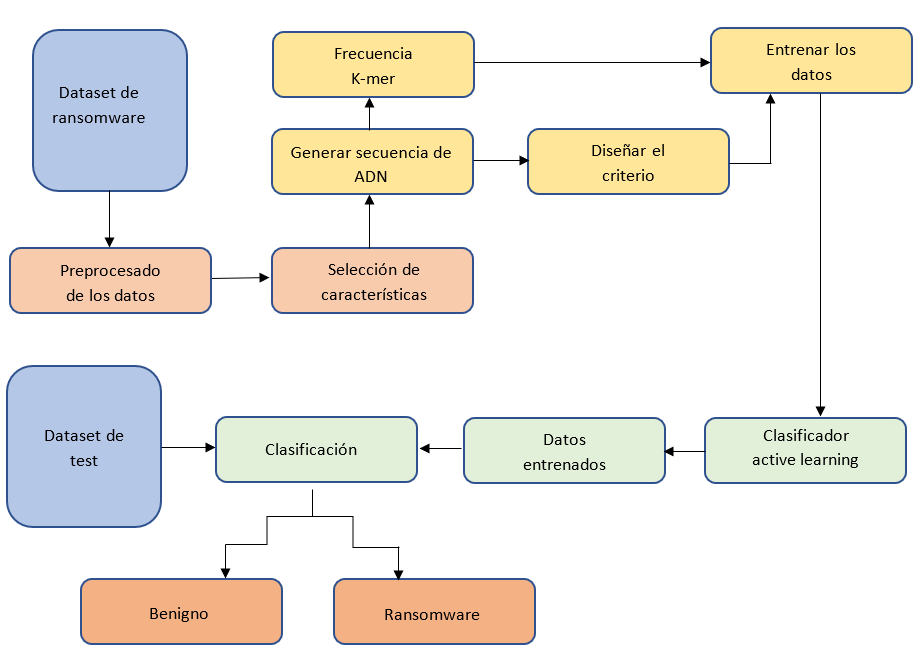
\includegraphics{images/adn.png}}}
\end{center}
\caption{Diagrama de secuencia del proyecto}
\label{fig:adn}
\end{figure}
El \gls{DNA} se usa para construir proteínas y otros componentes celulares de los seres vivos. Está compuesta por largas cadenas conformadas por las bases nitrogenadas: Adenina (A), Guanina (G), Citosina (C) y Timina (T).  Para la creación de la secuencia de \gls{DNA} digital, se realiza una correspondencia binaria para mapear estas moléculas como se observa en la Tabla \ref{tab:moleculas}.


\begin{table}[htb!]
    \centering
    \scriptsize %para hacer la tabla mas pequeña
    \caption{Mapeo de las bases nitrogenadas en código binario}
    \begin{tabular}{|m{3cm} | m{3cm}|}
        \hline
        \rowcolor[HTML]{C0C0C0} 
        \textbf{Codificación} & \textbf{Moléculas}\\ \hline
        00 & A\\ \hline
        01 & C \\ \hline
        10 & G\\ \hline
        11 & T\\ \hline
    \end{tabular}
    \label{tab:moleculas}
\end{table}

Posteriormente, se generan secuencias de \gls{DNA} digital de manera aleatoria para entrenar un modelo de \gls{ML}. Se utiliza \textit{active learning}, un método por el que se pueden realizar consultas de manera interactiva para etiquetar nuevos datos con su salida deseada. Finalmente, se usan algoritmos de clasificación (\gls{NB}, \gls{RF} y Optimización Mínima Secuencial) para detectar las familias de ransomware. 

El \textit{dataset} utilizado se compone de 1524 muestras, de las cuales 582 pertenecen a ransomware y 942 a goodware, con un total de 30970 características.

\subsection{Trabajos que Utilizan Llamadas a la API de Windows}

\noindent En esta sección se agrupan los trabajos que usan las llamadas a la \gls{API} de Windows como característica para desarrollar sus modelos, al igual que este trabajo.

Daniele Sgandurra \textit{et al.} (2016) \cite{elderan} presentan EldeRan, un sistema que usa un algoritmo de aprendizaje automático para clasificar y analizar ransomware dinámicamente. EldeRan se basa en la observación de que las muestras de ransomware suelen realizar acciones que son únicas o significativas con respecto a las realizadas por un programa benigno. Por lo tanto, EldeRan monitoriza los programas sospechosos en sus primeras fases de instalación en un entorno controlado con Cuckoo Sandbox, comprobando si sus acciones coinciden con las que haría un ransomware. La Figura \ref{fig:elderan} representa este sistema. Analizan un conjunto de datos descargados de VirusShare que contiene 582 muestras de ransomware pertenecientes a 11 familias y 942 aplicaciones benignas. A partir de estos datos, se analizan las siguientes características: llamadas a la \gls{API} de Windows, operaciones de clave de registro y del sistema de archivos (lectura, apertura, escritura y eliminación), el conjunto de operaciones realizadas con cierta extensión, operaciones de directorio, archivos eliminados (es decir, el conjunto de archivos que se eliminan por una aplicación durante su instalación) y las cadenas de caracteres incrustadas en el archivo. Todas las funciones, excepto las cadenas, se recopilan mientras se analiza dinámicamente el ransomware. Después de esta fase de análisis, se aplica un algoritmo de selección de características para seleccionar las más relevantes. Por último, las matrices que contienen estas características se utilizan en un clasificador \gls{LR} regularizado que devuelve si es ransomware o un archivo benigno. EldeRan no se basa en firmas, por lo que no necesita tener conocimientos previos de ransomware y puede detectar nuevas familias. Comparan EldeRan con los algoritmos \gls{SVM} y \gls{NB} y demuestran que el rendimiento máximo de estos algoritmos se alcanza con 400 características. Por lo tanto, agregar más características no mejora la precisión, por lo que la selección de características es importante para reducir la complejidad de los algoritmos de aprendizaje automático sin afectar el rendimiento. EldeRan alcanza un área bajo la curva \gls{ROC} del 99,5\% y tiene una tasa de fallos de 2,4\%, inferior a la de \gls{SVM} (4,2\%) y \gls{NB} (8,0\%).

\begin{figure}[h!]
\begin{center}
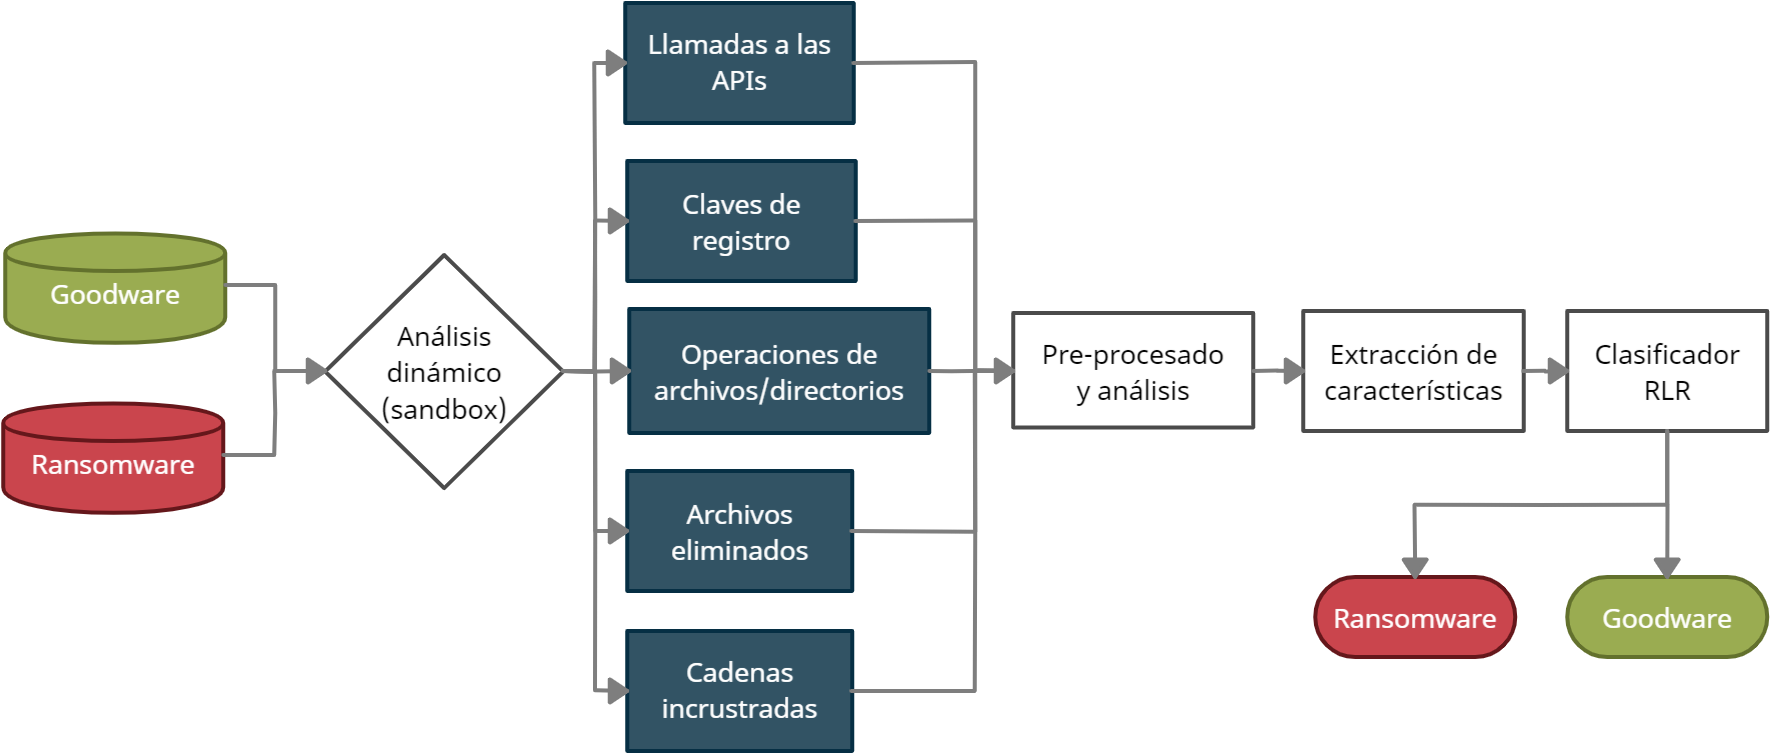
\includegraphics[width=1\linewidth]{images/elderan.png}
\end{center}
\caption{Representación del sistema EldeRan \cite{elderan}}
\label{fig:elderan}
\end{figure}

\newpage

Zhi-Guo Chen \textit{et al.} (2017) \cite{flow} proponen un sistema dinámico representado en la Figura \ref{fig:flow} que utiliza gráficos de flujo de llamadas \gls{API} (\gls{CFG}) y algoritmos como \gls{RF}, \gls{SVM}, \gls{NB} y \gls{LR} para detectar programas ransomware conocidos y desconocidos. Este sistema utiliza la herramienta \textit{API Monitor} para recopilar los datos de las llamadas a las \gls{API} que realiza el programa sospechoso cuando se ejecuta en una máquina virtual. Después, el sistema genera los \gls{CFG} para representar el comportamiento del programa y convierte estos gráficos en vectores de características etiquetados. Posteriormente selecciona el mínimo número de características para reducir el tiempo de la fase de aprendizaje y mejorar el rendimiento. Por último, se usan los algoritmos anteriormente mencionados para construir el modelo de detección que prediga si un programa es ransomware o no, entrenándolo con los vectores de características generados. 

\begin{figure}[h!]
\begin{center}
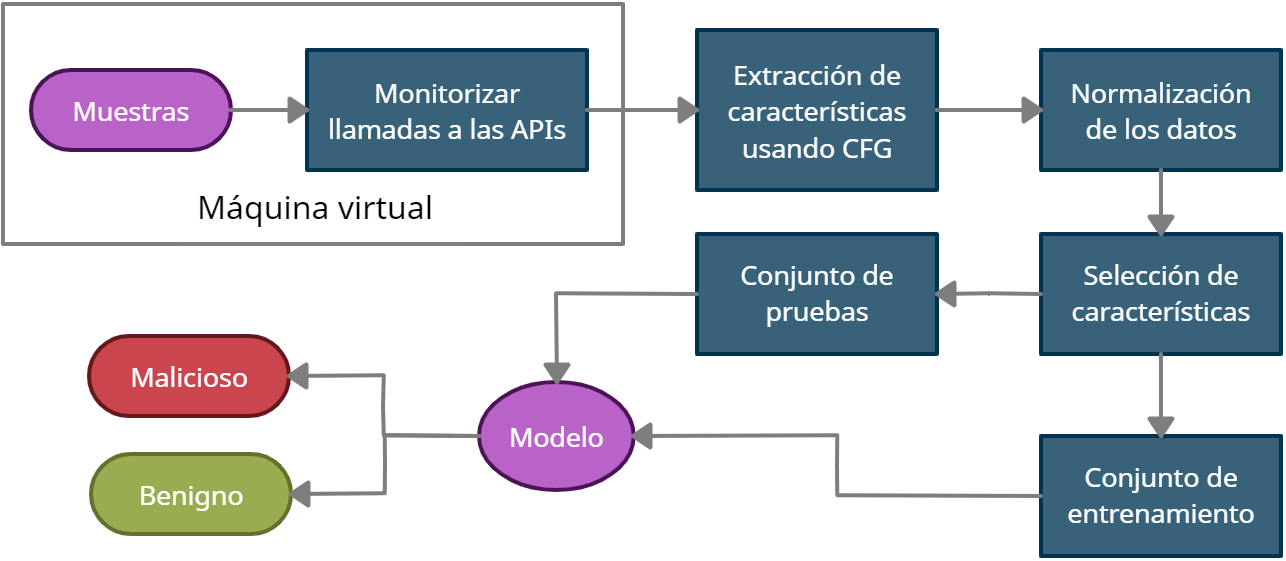
\includegraphics[width=0.9\linewidth]{images/flow.png}
\end{center}
\caption{Representación del sistema dinámico de detección de ransomware \cite{flow}}
\label{fig:flow}
\end{figure}

Hacen uso de la validación cruzada de k iteraciones (\textit{K-fold cross-validation}) para entrenar y probar el modelo. Esta validación consiste en dividir aleatoriamente el conjunto de datos original en k subconjuntos de igual tamaño, usando los k-1 conjuntos para el entrenamiento y el conjunto restante para las pruebas. Este proceso se repite k veces para que todos los subconjuntos se usen para las pruebas una vez. En este trabajo, se realiza la validación con k = 10. Tras varios experimentos, los mejores resultados se obtienen cuando se normalizan los datos y se aplican criterios de correlación y ganancia, obteniendo un 98,2\% en precisión (\textit{accuracy}) y un 97,6\% en \gls{TPR} con el algoritmo \gls{LR}. En cuanto al conjunto de datos usado, recopilan 83 muestras de ransomware diferentes y 85 muestras de software benigno.


Vinayakumar R \textit{et al.} (2017) \cite{shallow} proponen un sistema con una red neuronal profunda, en específico un perceptrón multicapa (\gls{MLP}), para la detección y clasificación de ransomware, usando las llamadas a las \gls{API}, algo que usan todos los trabajos. Analizan 7 familias de ransomware diferentes que han sacado de diversas fuentes, como Open Malware, Contagio Malware Dump, Malwr, theZoo, VirusTotal y VirusShare, recopilando un total de 755 muestras de ransomware y 219 de software benigno. Consideran alrededor de 131 llamadas \gls{API} sacadas de los registros de Cuckoo Sandbox tras analizar las muestras con dicha herramienta. La red \gls{MLP} es una función parametrizada, lo que significa que la \gls{TPR} de ransomware depende de los parámetros óptimos, la cantidad de capas ocultas, número de unidades, la tasa de aprendizaje, etc. Todos los experimentos con \gls{MLP} se realizan en tres capas con 1000, 500 y 250 unidades y se ejecutan con 500 ciclos de aprendizaje (llamados \textit{epochs}), con una tasa de aprendizaje entre 0,01 y 0,5. Este sistema alcanza una precisión (\textit{accuracy}) de 1,0 para detectar si un programa es ransomware o no.

Yuki Takeuchi \textit{et al.} (2018) \cite{detectingSVM} proponen un sistema de detección de ransomware utilizando máquinas de soporte vectorial (\gls{SVM}) y transformando las llamadas \gls{API} que realiza en ransomware en un conjunto de datos vectoriales. A diferencia de las soluciones existentes, este sistema propuesto analiza en profundidad el historial de llamadas a las \gls{API} con más detalle, demostrando una mejora en la \gls{TPR} correcta de ransomware. Usan \gls{SVM} porque generalmente tiene una generalización más alta que los otros algoritmos. La generalización es la capacidad de predecir datos desconocidos, y en este caso es muy útil para detectar ransomware desconocido, ya que no siempre se tienen muestras de todos los tipos posibles de ransomware. Ejecutan 276 muestras de ransomware y 312 muestras de programas benignos o \textit{goodware} en un entorno controlado y seguro con Cuckoo Sandbox, como se ha visto en anteriores trabajos. Después de la ejecución, Cuckoo Sandbox genera reportes que no solo contienen las llamadas a la \gls{API} de Windows, sino también los accesos a los archivos, los árboles de procesos, etc. A partir de estos reportes, solo se extraen las llamadas a la \gls{API} y se guardan como vectores que serán usados en \gls{SVM}. Para evaluar el sistema, usan la métrica de precisión (\textit{accuracy}) y obtienen un 97,48\%. También calculan la tasa de fallos, que es el número de falsos negativos (\gls{FN}) entre el número total de muestras, obteniendo un 1,64\%.

Seong Il Bae \textit{et al.} (2019) \cite{detecting} proponen un sistema de detección de ransomware en un entorno virtual en Windows 7 utilizando VMware que pueda distinguir entre ransomware y archivos benignos, así como entre ransomware y malware. Afirman que los métodos de detección de malware basados en firmas tienen dificultades para detectar ataques de día cero, por lo que no son adecuados para proteger los archivos de los usuarios. Por lo tanto, plantean un nuevo mecanismo de protección especializado que se centra en operaciones específicas de ransomware para poder diferenciarlos de otros malware y archivos benignos. La Figura \ref{fig:detecting} muestra el diagrama de flujo del sistema propuesto. En este trabajo extraen las secuencias de invocación de la \gls{API} de Windows mediante la herramienta intel PIN tool que realizan 1000 archivos de ransomware, 900 archivos de malware y 300 archivos ejecutables benignos. Si el tamaño del reporte de las llamadas es inferior a 10 KB, el reporte se descarta, ya que consideran que el archivo no se ejecutó correctamente. Con esa información generan los vectores de características utilizando un conjunto de n-grama, una subsecuencia de n elementos, y valores de \gls{CF-NCF}, un indicador para modelos de clasificación basado en \gls{TF-IDF}, que es un algoritmo que permite medir la importancia de una palabra en un conjunto de documentos. El rango del valor n de n-grama es entre 1 y 4, ya que comentan que las matrices se vuelven demasiado grandes para ser calculadas cuando n es mayor a cuatro. Posteriormente usan seis algoritmos de aprendizaje automático para crear su modelo de \gls{ML} con los vectores de características generados. Los seis algoritmos que utilizan son: \gls{RF}, \gls{LR}, \gls{NB}, descenso de gradiente o \gls{SGD}, \gls{KNN} y \gls{SVM}. Se realiza una validación cruzada a los datos de entrenamiento, que constituyen el 80\% del \textit{dataset}, y a los de test, el 20\% restante. Dichos procesos de entrenamiento y test fueron repetidos 5 veces. Al realizar sus experimentos con todos los algoritmos, consiguen una precisión (\textit{accuracy}) de entre 97\% y 98,65\%.

\begin{figure}[h!]
\begin{center}
{\scalebox{.3}{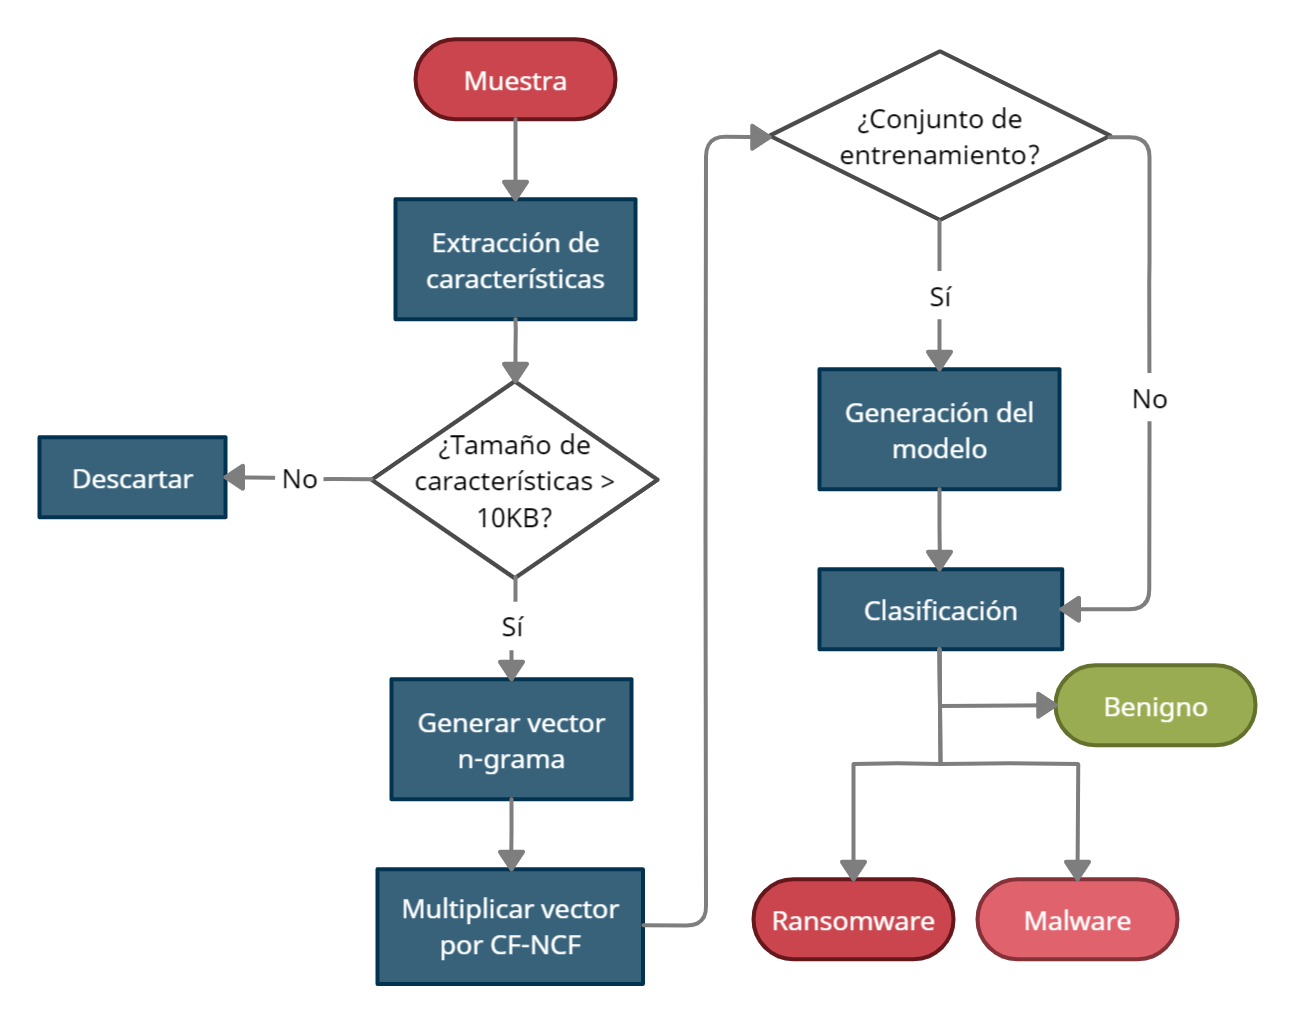
\includegraphics{images/detecting.png}}}
\end{center}
\caption{Diagrama de flujo del sistema propuesto \cite{detecting}}
\label{fig:detecting}
\end{figure}

Mahadevan Supramaniam \textit{et al.} (2019) \cite{Kok2019} proponen un sistema de dos fases que detecta cripto-ransomware antes de que pueda cifrar los archivos del usuario. Las dos fases son:

\begin{itemize}
    \item \textbf{Algoritmo de aprendizaje}: El archivo de muestra se introduce en Cuckoo Sandbox, el cual extrae las llamadas a las \gls{API} de Windows de cifrado (un total de 232). Posteriormente se analizan utilizando un algoritmo de aprendizaje que determina si el programa sospechoso es un cripto-ransomware o no. Este algoritmo selecciona características de forma aleatoria para generar árboles de decisión, ya que hay una gran cantidad de llamadas a las \gls{API} y esto causa \textit{overfitting} o ``sobreajuste''. Si el programa es un cripto-ransomware, el algoritmo genera una firma del programa malicioso y envía una notificación a un repositorio de firmas. 
    
    \item \textbf{Repositorio de firmas}: Una vez que se ha clasificado la muestra, se almacena un la firma de ella utilizando el algoritmo \gls{RSA} en una base de datos \gls{SQL}. La finalidad es que, cuando se vaya a ejecutar un archivo, primero se compruebe en la base de datos, de forma más rápida y eficiente, mediante consultas \gls{SQL}. Tener este repositorio permite la detección de las amenazas en una etapa mucho más temprana, aunque solo puede detectar cripto-ransomware conocido.
\end{itemize}

Las dos fases de este sistema, el cual está representado en la Figura \ref{fig:peda}, forman dos capas de detección temprana para cripto-ransomware, garantizando al usuario que no va a perder ningún archivo. En este trabajo se centran en la primera fase, desarrollando un algoritmo de aprendizaje al que llaman PEDA, obteniendo una \gls{TPR} del 98,72\%, un \gls{AUC} del 99,3\% y una tasa de falsos positivos (\gls{FPR}) un 1,56\% más baja en comparación con los algoritmos \gls{NB}, \gls{RF}, una mezcla de los dos anteriores (método de ensemble) y con el algoritmo EldeRan desarrollado en \cite{elderan}. Usan un \textit{dataset} extraído por el \gls{RISS} en 2016, que contiene datos de \gls{API} de 10 familias de ransomware y de software benigno, en concreto 582 muestras de ransomware y 942 de software benigno.


\begin{figure}[h!]
\begin{center}
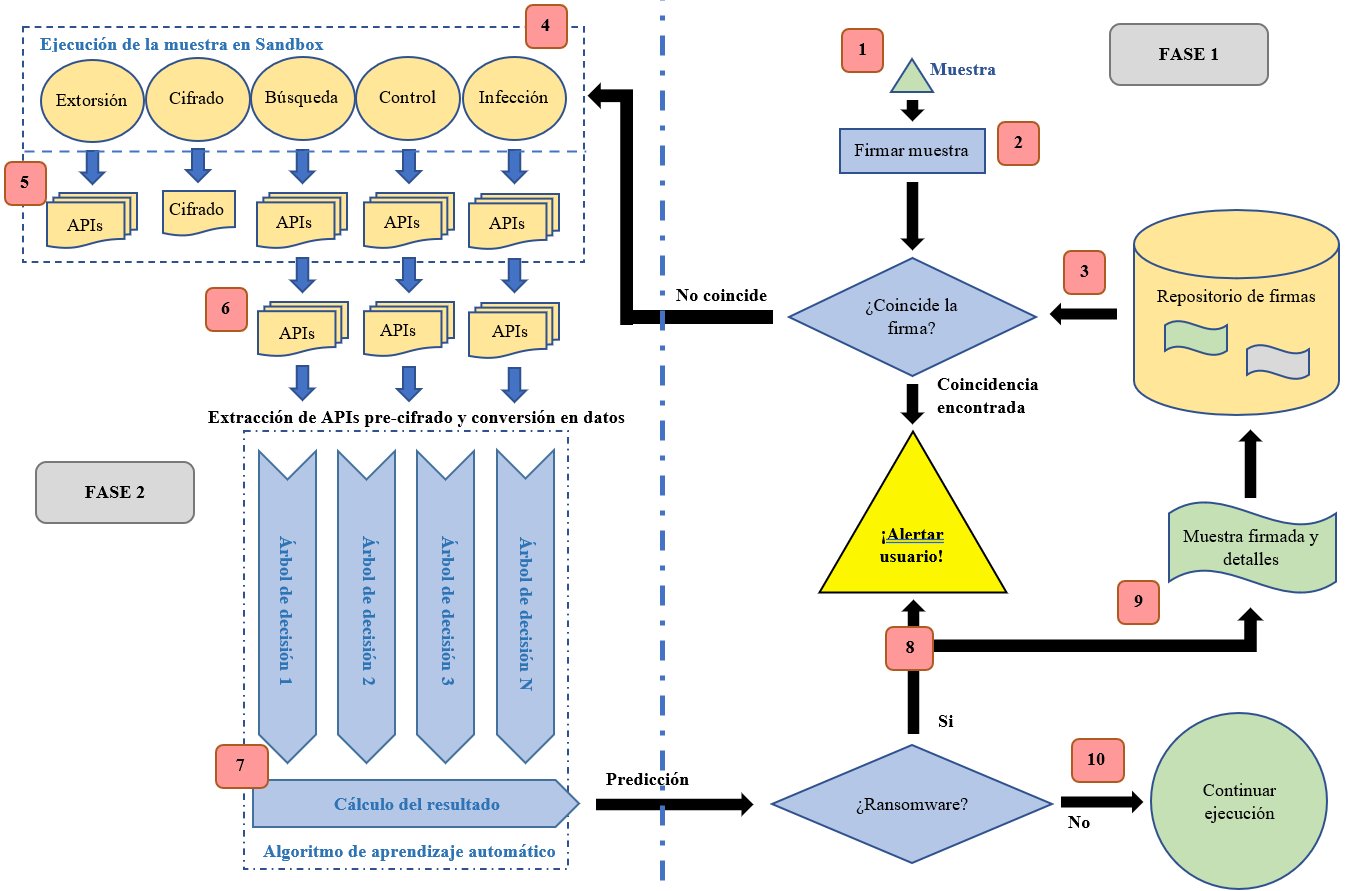
\includegraphics[width=1\linewidth]{images/peda.PNG}
\end{center}
\caption{Modelo del sistema propuesto por \cite{Kok2019}}
\label{fig:peda}
\end{figure}

\newpage

Brijesh Jethva \textit{et al.} (2019) \cite{entropy} propone un sistema de detección de ransomware dinámico mediante la combinación de un modelo de aprendizaje automático con modelos de entropía y firmas de archivos. Con este nuevo enfoque, se observa que el objetivo del ransomware son áreas específicas de claves de registro y su ejecución implica operaciones de alta entropía en extensiones de archivo desconocidas. Las características más seleccionadas son las llamadas a la \gls{API} y las claves de las operaciones de registro, pero la presencia de otras características como las bibliotecas de enlaces dinámicos (\gls{DLL}), los directorios accedidos, las líneas de comando, cadenas insertadas, etc. Con todas estas características, se seleccionan las más importantes con la ayuda de métodos de selección de características para evitar el \textit{overfitting} o sobreajuste para posteriormente clasificarlas mediante técnicas de aprendizaje automático, que son \gls{SVM}, \gls{LR} y \gls{RF}. Para realizar el estudio, utilizan un conjunto de datos que consta de 666 muestras de ransomware y 103 archivos benignos. Para balancear estos datos, usan la técnica \gls{SMOTE}, la cual utiliza el algoritmo \gls{KNN} para generar datos nuevos para las clases con menos muestras. En este caso, se generan datos para ambas clases, obteniendo 1.072 muestras de cada una. En los experimentos, el algoritmo que mejor rendimiento tiene es el de \gls{LR}, obteniendo una \gls{TPR} del 100\%, una precisión (\textit{accuracy}) del 98,7\% y una tasa de falsos positivos del 1,41\%.


Jinsoo Hwang \textit{et al.} (2020) \cite{two} proponen un modelo de detección de ransomware con dos etapas. La primera etapa es un modelo de Markov constituido por dos cadenas de Markov, una para ransomware y la otra para programas benignos. Una cadena de Markov se crea con un espacio de estados y una matriz de probabilidades de transición. El espacio de estado abarca todas las llamadas a la \gls{API} de Windows realizadas tanto por las muestras de ransomware como por las de \textit{goodware}. Estas cadenas se utilizan para decidir si la muestra entrante es ransomware o no, comparando las probabilidades de que una muestra pertenezca a cada clase. La segunda etapa consiste en un modelo de aprendizaje automático, usando \gls{RF} para controlar la tasa de falsos negativos (\gls{FNR}) que devuelve el modelo de Markov, ya que es bastante alta (20\%). Para los experimentos, recopilan 1909 muestras de ransomware de VirusShare y 1139 muestras de \textit{goodware} de Softonic, ejecutándolas dentro de Cuckoo Sandbox para obtener los reportes de donde extraen la secuencia de llamadas a las \gls{API}. Al final de las dos etapas, obtienen una precisión (\textit{accuracy}) del 97,3\%, una tasa de falsos positivos (\gls{FPR}) del 4,8\% y una tasa de falsos negativos (\gls{FNR}) del 1,5\%.


S.H. Kok \textit{et al.} (2020) \cite{Kok2020} proponen un sistema que detecte cripto-ransomware antes de que entre en la etapa de cifrado de archivos (\gls{PEDA}). \gls{PEDA} proporciona dos niveles de detección: el primer nivel consiste en una comparación de firmas, generadas con \gls{SHA}-256. Se compara la firma del archivo sospechoso con firmas de diferentes tipos de ransomware conocidos almacenadas en un repositorio MySQL. Si coinciden los \textit{hashes}, se alerta al usuario de que el archivo es un ransomware. Si no, \gls{PEDA} entra en la segunda etapa, que consiste en enviar ese archivo a Cuckoo Sandbox para que lo analice y obtenga el reporte de su comportamiento. De ese reporte se extraen las \gls{API} que se llaman antes de que empiece el proceso de cifrado, por lo que el algoritmo sacará todas las \gls{API} hasta que encuentre una que empiece por ``crypt''. Se identifican 14 \gls{API}s importantes para diferenciar entre ransomware y goodware, con 3 de ellas encontradas en la mayor parte de ransomwares. Posteriormente las \gls{API} extraídas (232 en total) se guardarán en un archivo de valores separados por comas (\gls{CSV}), el cual se introducirá en el algoritmo de aprendizaje automático \gls{RF} para que prediga si el archivo sospechoso es un ransomware o no. Si la predicción lo identifica como ransomware, \gls{PEDA} pondrá en cuarentena el archivo, alertará al usuario y almacenará su firma en el repositorio MySQL de firmas. La Figura \ref{fig:peda2} muestra el flujo de datos del sistema \gls{PEDA}. Para entrenar el modelo de \gls{ML}, utilizan tres \textit{datasets} con un total de 942 muestras de \textit{goodware} y 1691 muestras de ransomware de VirusShare y theZoo. El modelo obtiene una exhaustividad (\textit{recall}) del 99,9\% con validación cruzada de 10 iteraciones en dos de las tres \textit{datasets}, usando un ratio de entrenamiento:prueba 80:20. En cuanto a las limitaciones, \gls{PEDA} tiene una importante dependencia de uso de las \gls{API}s de Windows, lo que supone que no sería capaz de detectar ransomware que utilice su propio código nativo de cifrado, lo que convierte este algoritmo en un suplemento para la detección de ransomware y no un sistema completo para ello.

\begin{figure}[htb]
\begin{center}
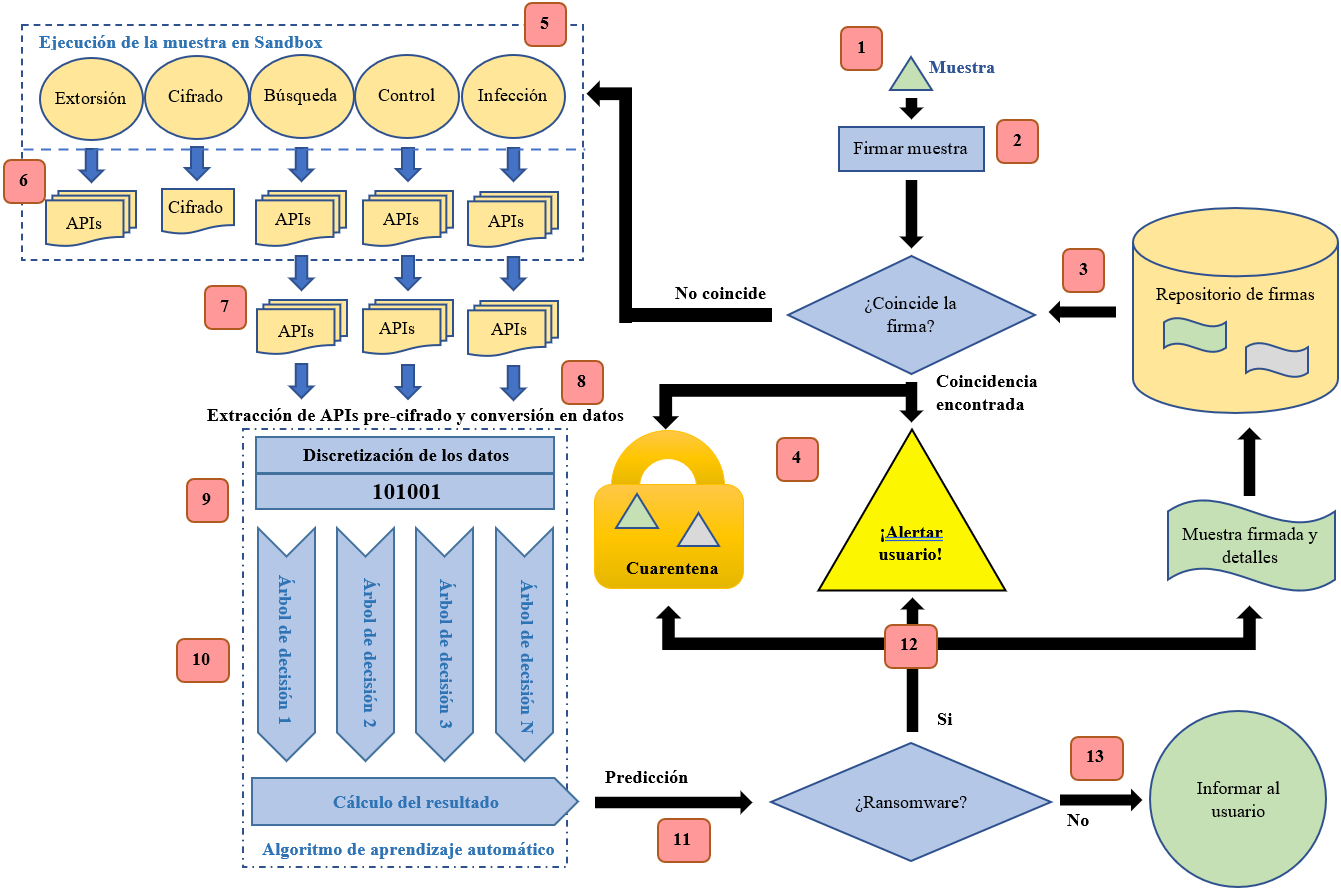
\includegraphics[width=1\linewidth]{images/peda2.PNG}
\end{center}
\caption{Representación del flujo de datos del sistema PEDA propuesto por S.H. Kok \textit{et al.} \cite{Kok2020}}
\label{fig:peda2}
\end{figure}

La detección basada en el análisis del comportamiento se basa en identificar cambios relevantes en el sistema. Abdullahi Arabo \textit{et al.} en \cite{ARABO2020289} (2020) desarrollaron un programa que recopila del sistema las llamadas a \gls{DLL} de \gls{API}, el uso de los recursos del sistema, y los archivos utilizados por  los procesos. Dicha información se discretiza y posteriormente toma dos caminos: a una solución de \gls{ML}, utilizando árboles de decisión, \gls{RF} y redes neuronales, que será capaz de detectar ransomware después del suficiente entrenamiento, y a un sistema de detección mediante umbrales, debido a que no cualquier tipo de datos, como las cadenas, pueden ser introducidos a una solución de \gls{ML}.

La detección del ransomware se lleva a cabo mediante un \textit{script} de Python. Se ejecutan ataques ransomware en una máquina virtual Windows 7, que destruirían dicho \textit{script} con la información que ha recopilado, así que, dicha máquina está conectada con otra base Linux mediante un canal seguro para el paso de la información. Se crean dos hilos principales diferenciados porque hay datos que no tardan el mismo tiempo en ser obtenidos: Hilo ``analysis'', que recoge datos variables en bucle hasta el final del proceso y el  Hilo ``info'', el cual recoge datos constantes, los manda y finaliza.También existen otros tres para leer el nombre de los ficheros,y reconocer su extensión, puesto que los datos cifrados de forma maligna adaptan extensiones reconocibles(p.e.: .wncry), los \textit{tagfiles} y para los datos que son muy lentos de obtener. Se utiliza también el programa Tiny tracer: cuando se ejecuta un programa con él, genera un archivo con todas las llamadas a \gls{DLL} de \gls{API}.

Se crea un sistema basado en media de pesos para reconocer si un dato detecta el ransomware o no. Los datos son procesados por funciones, que tienen un cierto umbral: si lo sobrepasan devolverán 1, por el contrario 0, y se compara con un coeficiente, que depende del umbral y la función. Al final, todos estos valores se utilizan para elaborar una media. Si es por encima de 0,5 es sospechoso de ser malicioso y salta un pop-up al usuario para permitir matar al proceso.

Sana Aurangzeb \textit{et al.} (2021) \cite{Aurangzeb2021} exponen un trabajo basado principalmente en el análisis dinámico enfocado a los \gls{HPC}, que son variables propias de la actividad del hardware como por ejemplo ciclos de reloj, accesos a caché, fallos de caché, instrucciones de salto tomadas, etc. En este estudio se utilizan 11 variables \gls{HPC} para la clasificación de ransomware, que se hará entre ransomware y non-ransomware, siendo non-ransomware muestras de malware y no de goodware. Esto se debe ya que se el ransomware está considerado uno de los tipos de malware que mayor daño provocan en términos financieros. 
A la hora de construir el \textit{dataset}, se obtienen 160 muestras de malware de VirusShare y tras un análisis estático en la misma plataforma se etiquetan como ransomware o non-ransomware. Una vez obtenidas las muestras, se ejecutan en un entorno seguro y se recoge la información relativa a los \gls{HPC}. Para asegurar la precisión y corrección de los datos se ejecuta cada muestra tres veces en una máquina virtual. Los 11 \gls{HPC} recogidos para entrenar el modelo son \textit{task clock}, \textit{context switching}, \textit{\gls{CPU} utilized}, \textit{\gls{CPU} migrations}, \textit{page faults}, \textit{\gls{CPU} cycles}, \textit{cache-misses}, \textit{instruction retires}, \textit{branch taken}, \textit{branch-misses} y \textit{execution time}. Con estas variables se construye una matriz de correlación para seleccionar los atributos concretos a utilizar y así ahorrar costes computacionales.
Para el entrenamiento de los datos se utiliza un 80\% del \textit{dataset} y el resto son usados para prueba. Además, se utiliza el método \textit{k-fold cross-validation}.
En la Figura \ref{fig:im13} se puede ver el flujo del proceso de entrenamiento y prueba.
Se utilizan cuatro modelos de clasificación, árboles de decisión (ofrece una precisión de 0,94), bosques aleatorios (precisión de 0,97), potenciación de gradiente (precisión de 0,94) y potenciación extrema de gradiente (ofrece una precisión de 0,97).
Las conclusiones obtenidas de este estudio es que existe la posibilidad de explotar características hardware para la detección de ransomware. Por otro lado, como no se trabaja con muestras benignas, se desconoce el comportamiento que tendrá el uso de estas características para detectar ransomware, además, la recogida de características es específica de un sistema con una configuración hardware determinada, lo que implica que si el sistema en el que se recogen los datos tiene otra arquitectura, el modelo no será aplicable.

\begin{figure}[htb]
\begin{center}
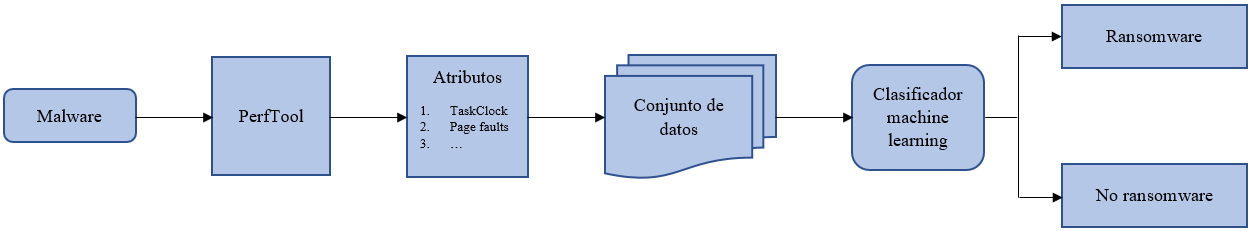
\includegraphics[width=1\linewidth]{images/hpc.PNG}
\end{center}
\caption{Flujo del proceso de entrenamiento y prueba.}
\label{fig:im13}
\end{figure}


A continuación se muestra una Tabla \ref{tab:estadoarte} comparativa de los trabajos previamente mencionados que usan la extracción de \gls{API}s para la detección de malware y ransomware, exponiendo de manera clara qué algoritmos de aprendizaje automático utilizan, qué datos usan y qué resultados obtienen:

{\footnotesize
\begin{longtable}{|p{0.11\textwidth}|p{0.13\textwidth}|p{0.3\textwidth}|p{0.35\textwidth}|}
\caption{Tabla comparativa de los trabajos que usan aprendizaje automático para detectar malware mediante la extracción de APIs.}
\label{tab:estadoarte}
\\
\hline
\rowcolor[HTML]{C0C0C0} 
\multicolumn{1}{|c|}{\cellcolor[HTML]{C0C0C0}{\color[HTML]{000000} \textbf{Trabajo}}} &
\multicolumn{1}{c|}{\cellcolor[HTML]{C0C0C0}{\color[HTML]{000000} \textbf{Algoritmos}}} &
\multicolumn{1}{c|}{\cellcolor[HTML]{C0C0C0}{\color[HTML]{000000} \textbf{Conjuntos de datos}}} &
\multicolumn{1}{c|}{\cellcolor[HTML]{C0C0C0}{\color[HTML]{000000} \textbf{Resultados}}} \\ \hline
\endfirsthead

\hline
\rowcolor[HTML]{C0C0C0} 
\multicolumn{1}{|c|}{\cellcolor[HTML]{C0C0C0}{\color[HTML]{000000} \textbf{Trabajo}}} &
\multicolumn{1}{c|}{\cellcolor[HTML]{C0C0C0}{\color[HTML]{000000} \textbf{Algoritmos}}} &
\multicolumn{1}{c|}{\cellcolor[HTML]{C0C0C0}{\color[HTML]{000000} \textbf{Conjuntos de datos}}} &
\multicolumn{1}{c|}{\cellcolor[HTML]{C0C0C0}{\color[HTML]{000000} \textbf{Resultados}}} \\ \hline
\endhead

\cite{automatic} (2011)    &
  - Hierarchical clustering (agrupamiento jerárquico) \newline - Nearest prototype classifier &
  - 3.133 muestras de clases conocidas de malware de CWSandbox \newline - 33.698 muestras de clases desconocidas de malware de Sunbelt Software &
  - Precisión: 99,6\% \newline - Valor-F: 95\%. \\ \hline
\cite{zero} (2011)    &
  - \gls{NB} \newline - \gls{KNN} \newline - \gls{DT} \newline - \gls{SVM} &
  - 51.223 muestras de malware del proyecto Honeynet y VX Heaven \newline - 15.480 muestras de goodware &
  - \gls{DT}: \gls{TPR} 93\%, \gls{FPR} 6,8\%, Precisión 93,1\%, Valor-F 93\%, Area \gls{ROC} 93,1\% \newline - \gls{KNN}: \gls{TPR} 94,8\%, \gls{FPR} 5,1\%, Precisión 94,8\%, Valor-F 94,8\%, Area \gls{ROC} 96,6\% \newline - \gls{NB}: \gls{TPR} 91\%, \gls{FPR} 9\%, Precisión 91\%, Valor-F 91\%, Area \gls{ROC} 93,8\% \newline - \gls{SVM} PolyKernel normalizado: \gls{TPR} 98,6\%, \gls{FPR} 2,5\%, Precisión 97,8\%, Valor-F 98,6\%, Area \gls{ROC} 98,2\% \newline - \gls{SVM} PolyKernel: \gls{TPR} 93,4\%, \gls{FPR} 6,9\%, Precisión 93,6\%, Valor-F 93,4\%, Area \gls{ROC} 93,2\% \newline - \gls{SVM} Puk: \gls{TPR} 94\%, \gls{FPR} 6,4\%, Precisión 94\%, Valor-F 93,2\%, Area \gls{ROC} 93,9\% \newline - \gls{SVM} \gls{RBF}: \gls{TPR} 92,9\%, \gls{FPR} 7,3\%, Precisión 92,9\%, Valor-F 92,9\%, Area \gls{ROC} 92,8\% \\ \hline
\cite{ravimalware} (2012)  & 
    - \gls{NB} \newline - \gls{SVM} \newline - \gls{DT} \newline - Algoritmo clasificador propio de 4-gramas & 
    - 179 muestras de malware de VXHeavens \newline - 94 muestras de goodware de una instalación de Windows XP &
    Precisión: \newline - \gls{NB}: 48,69\% \newline - \gls{SVM}: 64,43\% \newline - \gls{DT}: 56,77\% \newline - Algoritmo propuesto: 90\%\\ \hline
\cite{elderan} (2016)      & 
    - \gls{NB} \newline - \gls{SVM} \newline - EldeRan & 
    - 582 muestras de ransomware de 11 familias de VirusShare \newline - 942 muestras de goodware de Software Informer &
    - EldeRan: \gls{AUC} 99,49\%, \gls{FPR} 1,61\%, \gls{TPR} 96,34\% \newline - \gls{SVM}: \gls{AUC} 99,29\%, \gls{FPR} 1,99\%, \gls{TPR} 92,19\% \newline - \gls{NB}: \gls{AUC} 96,96\%, \gls{FPR} 9,58\%, \gls{TPR} 94,53\% \\ \hline
\cite{shallow} (2017)      & 
    - \gls{MLP} \newline - \gls{LR} \newline - \gls{NB} \newline - \gls{DT} \newline - \gls{RF} \newline - \gls{KNN} \newline - \gls{SVM} & 
    - 755  muestras  de  ransomware de varias fuentes \newline -  219 muestras de goodware &
    - \gls{MLP}: Precisión 100\%, Exactitud 100\%, Exhaustividad 100\%, Valor-F 100\% \newline - \gls{LR}: Precisión 98,8\%, Exactitud 98,5\%, Exhaustividad 100\%, Valor-F 99,3\% \newline - \gls{NB}: Precisión 97,2\%, Exactitud 96,6\%, Exhaustividad 100\%, Valor-F 98,3\% \newline - \gls{DT}: Precisión 96,4\%, Exactitud 95,7\%, Exhaustividad 100\%, Valor-F 97,8\% \newline - \gls{RF}: Precisión 98,4\%, Exactitud 98\%, Exhaustividad 100\%, Valor-F 99\% \newline - \gls{KNN}: Precisión 96,8\%, Exactitud 96,2\%, Exhaustividad 100\%, Valor-F 99,3\% \newline - \gls{SVM}: Precisión 98,8\%, Exactitud 98,5\%, Exhaustividad 100\%, Valor-F 99,3\% \\ \hline
\cite{flow} (2017)         & 
    - \gls{NB} \newline - \gls{SVM} \newline - \gls{RF} \newline - \gls{LR} & 
    - 83 muestras de ransomware diferentes de VirusShare \newline - 85 muestras de goodware de Software Informer &
    - \gls{LR}: Precisión: 98,2\%, \gls{TPR} 97,6\%, \gls{FPR} 1,2\% \newline - \gls{SVM}: Precisión: 95,8\%, \gls{TPR} 96,4\%, \gls{FPR} 4,7\% \newline - \gls{RF}: Precisión: 95,8\%, \gls{TPR} 96,4\%, \gls{FPR} 4,7\% \newline - \gls{NB}: Precisión: 92,3\%, \gls{TPR} 94\%, \gls{FPR} 9,4\% \\ \hline
\cite{detectingSVM} (2018) & 
    - \gls{SVM} & 
    - 276 muestras de ransomware \newline - 312 muestras de goodware &
    - Precisión: 97.48\% \newline - Tasa de error: 1.64\% \\ \hline
\cite{detecting} (2019)    & 
    - \gls{RF} \newline - \gls{LR} \newline - \gls{NB} \newline - \gls{SGD} \newline - \gls{KNN} \newline - \gls{SVM} & 
    - 1000 muestras de ransomware \newline - 900 muestras de malware \newline - 300 muestras de goodware &
    - \gls{RF}: Precisión 98,39\%, Exhaustividad 98,55\%, Valor-F 98,56\%, Exactitud 98,58\% \newline - \gls{KNN}: Precisión 96,13\%, Exhaustividad 96,13\%, Valor-F 96,25\%, Exactitud 95,50\% \newline - \gls{NB}: Precisión 87,43\%, Exhaustividad 87,92\%, Valor-F 82,72\%, Exactitud 89,38\% \newline - \gls{SGD}: Precisión 93,96\%, Exhaustividad 90,95\%, Valor-F 90,22\%, Exactitud 91,61\% \newline - \gls{LR}: Precisión 90,08\%, Exhaustividad 93,99\%, Valor-F 92,98\%, Exactitud 92,07\% \newline - \gls{SVM}: Precisión 74,81\%, Exhaustividad 78,99\%, Valor-F 75,98\%, Exactitud 79,95\% \\ \hline
\cite{Kok2019} (2019)         & 
    - \gls{PEDA} \newline - \gls{RF} \newline - \gls{NB} \newline - Ensamble (\gls{RF}+\gls{NB}) & 
    - 582 muestras de ransomware \newline - 942 muestras de goodware \newline Los dos conjuntos de muestras fueron extraídos por el \gls{RISS} &
    - \gls{PEDA}: \gls{AUC} 99,30\%, \gls{FPR} 1,56\%, Precisión 97,05\%, \gls{TPR} 95\% \newline - \gls{RF}: \gls{AUC} 95\%, \gls{FPR} 7\%, Precisión 92\%, \gls{TPR} 91\% \newline - \gls{NB}: \gls{AUC} 81\%, \gls{FPR} 15\%, Precisión 83\%, \gls{TPR} 79\% \newline - Ensamble: \gls{AUC} 82,5\%, \gls{FPR} 16\%, Precisión 88\%, \gls{TPR} 98\% \\ \hline
\cite{entropy} (2019)      & 
    - \gls{SVM} \newline - \gls{RF} \newline - \gls{LR} & 
    Inicialmente: \newline - 666 muestras de ransomware \newline - 103 muestras de goodware \newline Para balancear los datos, usan \gls{SMOTE} y obtienen 1.072 muestras de cada clase &
    - \gls{SVM}: Precisión 98\%, Exhaustividad 97\%, Valor-F 97\% \newline - \gls{RF}: Precisión 97\%, Exhaustividad 97\%, Valor-F 97\% \newline - \gls{LR}: Precisión 97\%, Exhaustividad 97\%, Valor-F 97\% \newline \\ \hline
\cite{two} (2020)          & 
    - \gls{RF} & 
    - 1909 muestras de ransomware de VirusShare \newline - 1139 muestras de goodware de Softonic &
    - Precisión: 97,3\% \newline - \gls{FPR}: 4,8\% \newline - \gls{FNR}: 1,5\% \newline - Valor-F: 97,0\% \\ \hline
\cite{Kok2020} (2020)        & 
    - \gls{PEDA} (\gls{RF} discretizado) \newline - \gls{RF} & 
    Tres datasets: \newline - Dataset PE (con ransomware criptográfico): \newline 942 muestras de goodware \newline 205 muestras de cripto-ransomware \newline - Dataset Old (creada en 2016): \newline 942 muestras de goodware \newline 582 muestras de ransomware \newline - Dataset Full (PE + Old + nuevas muestras de VirusShare y theZoo ): \newline 942 muestras de goodware \newline 904 muestras de ransomware 
    \newline Tras obtener dicho dataset y realizar mediante el algoritmo de este estudio una limpieza de los datos para eliminar repetidos, el dataset restante obtenido es de 912 muestras &
    - Dataset PE: \newline \gls{PEDA}: \gls{TPR} 99,8\%, Precisión 99,9\%, Valor-F 99,9\%, \gls{ROC} 99,9\% \newline \gls{RF}: \gls{TPR} 99,6\%, Precisión 99,6\%, Valor-F 99,4\%, \gls{ROC} 99,5\% \newline - Dataset Old: \newline \gls{PEDA}: \gls{TPR} 95,6\%, Precisión 95,8\%, Valor-F 95,6\%, \gls{ROC} 98,5\% \newline \gls{RF}: \gls{TPR} 95,2\%, Precisión 95,2\%, Valor-F 95,2\%, \gls{ROC} 97,0\% \newline - Dataset Full: \newline \gls{PEDA}: \gls{TPR} 99,6\%, Precisión 99,6\%, Valor-F 99,4\%, \gls{ROC} 99,6\% \newline \gls{RF}: \gls{TPR} 99,7\%, Precisión 99,7\%, Valor-F 99,5\%, \gls{ROC} 99,5\% \\ \hline
\cite{ARABO2020289} (2020) & 
- \gls{NN} \newline
- \gls{KNN} \newline
- \gls{SVM} lineal\newline
- \gls{SVM} \gls{RBF} \newline 
- \gls{GP} \newline
- \gls{DT} \newline
- \gls{RF} \newline
- AdaBoost \newline
- \gls{QDA} \newline
- \gls{NB} &
- 41 aplicaciones benignas \newline
- 34 procesos malware, includios 7 muestras de ransomware &
Precisión: \newline
- \gls{NN}: 52,85\% \newline
- \gls{KNN}: 57,06\% \newline
- \gls{SVM} lineal: 63,05\% \newline
- \gls{SVM} \gls{RBF}: 60,50\%\newline 
- \gls{GP}: 59,8\% \newline
- \gls{DT}: 70,14\% \newline
- \gls{RF}: 75,01\% \newline
- AdaBoost: 61,64\% \newline
- \gls{QDA}: 62,7\% \newline
- \gls{NB}: 58,55 \%  \\ \hline
\cite{Aurangzeb2021} (2021) &
- \gls{DT} \newline
- \gls{RF} \newline
- Gradient Boosting \newline
- Extreme Gradient Boosting \newline&
 160 muestras de las cuales pertenecen 80 a ransomware y 80 a otros tipos de malware &
Precisión: \newline
- \gls{DT}: 94,5\% \newline
- \gls{RF}: 97\% \newline
- Gradient Boosting: 94,5\% \newline
- Extreme Gradient Boosting: 97\% \newline
Valor F: \newline
- \gls{DT}: 94\% \newline
- \gls{RF}: 97\% \newline
- Gradient Boosting: 94\% \newline
- Extreme Gradient Boosting: 97\% \newline
\gls{TPR}: \newline
- \gls{DT}: 88\% \newline
- \gls{RF}: 94\% \newline
- Gradient Boosting: 88\% \newline
- Extreme Gradient Boosting: 94\% \newline
\\ \hline


\end{longtable}}



